\chapter{Results}
\epigraph{The first law of thermodynamics says that work cannot be destroyed. We who use computers know better.}{A frustrated Ph.D. candidate}

\section{Periodic Orbits}

Four new periodic orbits P85, P60, P32 and P8 (\refFigsss{fig:p85}{fig:p60}{fig:p32}{fig:p8}) have been found, with periods $T= 85.50, 60.86, 32.00, 8.32$, for $\ReN = 400$, and periodic cell length $(\alpha,\gamma) = (2\pi/L_x,2\pi/L_z) = (1.14,1.67)$. This  set of cell parameters is known as the HKW cell. P85 and P60 were the first orbits found, and are in the fully symmetric subspace. P32 was the next orbit to be found, and is in the streamwise-asymmetric subspace $S_x$. P8 was the last orbit found, and is in the spanwise-asymmetric subspace $S_z$. I was unable to find any \ecs\ in the unconstrained phase space. 

\begin{figure}
\centerline{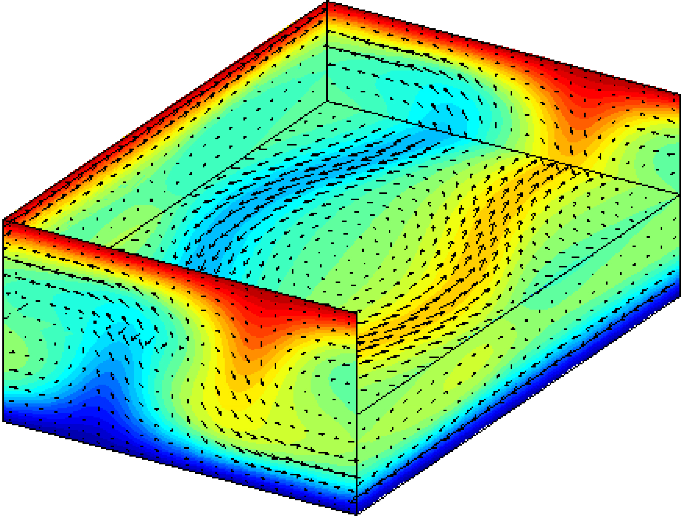
\includegraphics[width=\textwidth]{p85.pdf}}
\caption{A}\label{fig:p85}
\end{figure}

\begin{figure}
\centerline{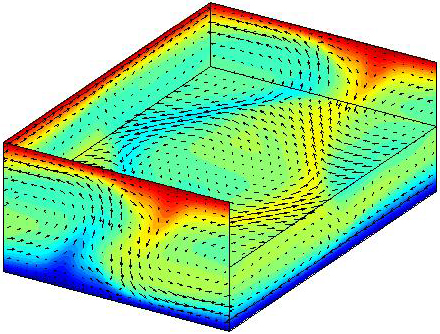
\includegraphics[width=\textwidth]{p60}}
\caption{B}\label{fig:p60}
\end{figure}


\begin{figure}
\centerline{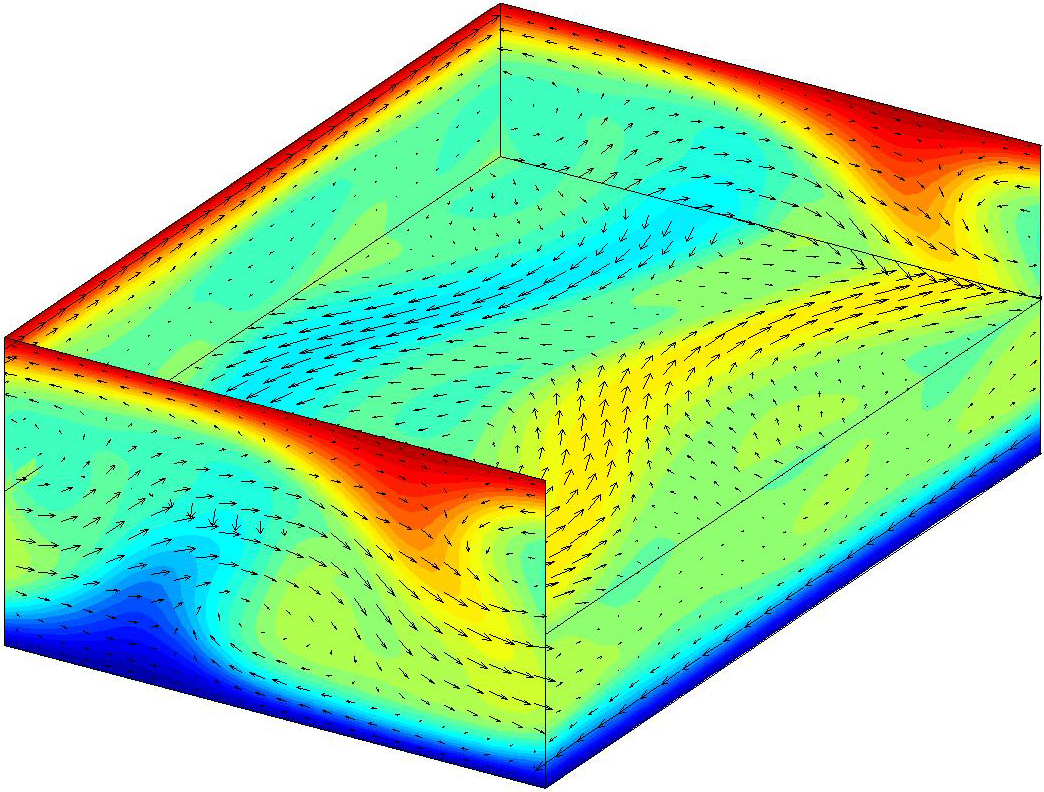
\includegraphics[width=\textwidth]{p32}}
\caption{C}\label{fig:p32}
\end{figure}


\begin{figure}
\centerline{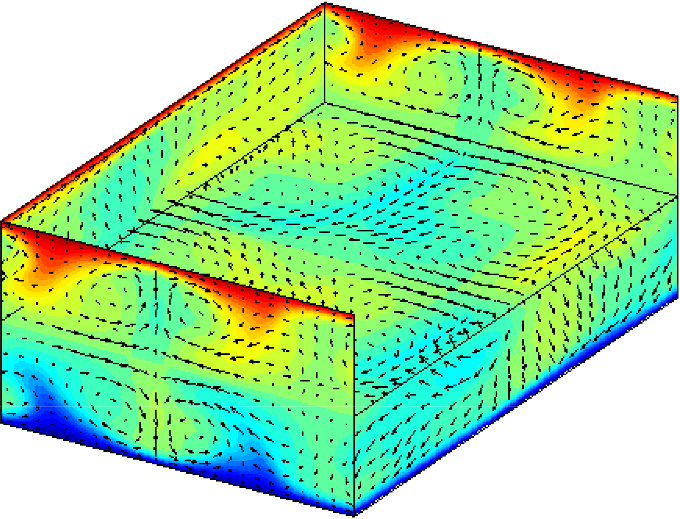
\includegraphics[width=\textwidth]{p8}}
\caption{D}\label{fig:p8}
\end{figure}

\subsection{Visualizations}   